\documentclass[10pt, titlepage, oneside, a4paper]{article}
\usepackage[T1]{fontenc}
\usepackage[english]{babel}
\usepackage{tikz}
\usetikzlibrary {positioning,fit}
\usepackage{amssymb, graphicx, fancyheadings}
\usepackage{amsmath}
\addtolength{\textheight}{20mm}
\addtolength{\voffset}{-5mm}
\renewcommand{\sectionmark}[1]{\markleft{#1}}

% \Section ger mindre spillutrymme, anv�nd dem om du vill
\newcommand{\Section}[1]{\section{#1}\vspace{-8pt}}
\newcommand{\Subsection}[1]{\vspace{-4pt}\subsection{#1}\vspace{-8pt}}
\newcommand{\Subsubsection}[1]{\vspace{-4pt}\subsubsection{#1}\vspace{-8pt}}
	
% appendices, \appitem och \appsubitem �r f�r bilagor
\newcounter{appendixpage}

\newenvironment{appendices}{
	\setcounter{appendixpage}{\arabic{page}}
	\stepcounter{appendixpage}
}{
}

\newcommand{\appitem}[2]{
	\stepcounter{section}
	\addtocontents{toc}{\protect\contentsline{section}{\numberline{\Alph{section}}#1}{\arabic{appendixpage}}}
	\addtocounter{appendixpage}{#2}
}

\newcommand{\appsubitem}[2]{
	\stepcounter{subsection}
	\addtocontents{toc}{\protect\contentsline{subsection}{\numberline{\Alph{section}.\arabic{subsection}}#1}{\arabic{appendixpage}}}
	\addtocounter{appendixpage}{#2}
}

% �ndra de rader som beh�ver �ndras
\def\inst{Computer Science}
\def\typeofdoc{Design Document}
\def\course{Distributed Systems 5DV147, 7.5p, HT15}
\def\pretitle{Gcom}
\def\title{Design proposal}
\def\adam{Adam Dahlgren}
\def\benj{Benjamin Sientzoff}
\def\userbenj{ens15bsf}
\def\useradam{dali}
\def\emailadam{\useradam{}@cs.umu.se}
\def\emailbenj{\userbenj{}@cs.umu.se}
\def\path{edu/5dv147/project/design/}
\def\graders{P-O \"{O}stberg, Ewnetu Bayuh Lakew, Ahmed Ali-Eldin}


% om du vill referera till katalogen d�r dina filer ligger kan du 
% anv�nda \fullpath som kommer att vara "~username/edu..." o.s.v.
\def\fullpath{\raisebox{1pt}{$\scriptstyle \sim$}\useradam/\path}


% H�r b�rjar sj�lva dokumentet
\begin{document}

	% skapar framsidan (om den inte duger: g�r helt enkelt en egen)
	\begin{titlepage}
		\thispagestyle{empty}
		\begin{large}
			\begin{tabular}{@{}p{\textwidth}@{}}
				\textbf{UME� UNIVERSITET \hfill \today} \\
				\textbf{Institution of \inst} \\
				\textbf{\typeofdoc} \\
			\end{tabular}
		\end{large}
		\vspace{10mm}
		\begin{center}
			\LARGE{\pretitle} \\
			\huge{\textbf{\course}}\\
			\vspace{10mm}
			\LARGE{\title} \\
			\vspace{15mm}
			\begin{large}
				\begin{tabular}{lp{4cm}}
					\textbf{Name} & \adam \hspace{0.6cm} \benj \\
					\textbf{E-mail} & \texttt{\emailadam}  \texttt{\emailbenj} \\
					\textbf{Path} & \texttt{\fullpath} \\
				\end{tabular}
			\end{large}
			\vfill
			\large{\textbf{Tutors}}\\
			\makebox[5pt]{\large{\graders}}
		\end{center}
	\end{titlepage}


	% fixar sidfot
	\lfoot{\footnotesize{\adam, \benj}}
	\rfoot{\footnotesize{\today}}
	\lhead{\sc\footnotesize\title}
	\rhead{\nouppercase{\sc\footnotesize\leftmark}}
	\pagestyle{fancy}
	\renewcommand{\headrulewidth}{0.2pt}
	\renewcommand{\footrulewidth}{0.2pt}

	\pagenumbering{roman}
	\tableofcontents
	
	% och l�gger in en sidbrytning
	\newpage

	\pagenumbering{arabic}

	\setlength{\parindent}{0pt}
	
	\setlength{\parskip}{10pt}

	\section{Problem}

\paragraph{}{
	GCom is a middle ware for group communication. It means,
 GCom has to be scallable and robust.
}

\subsection{Requirements}

\paragraph{Scallability}{
	To be scallable, GCom uses Peer to Peer based features.
 Typically, data is not centralized on a server but shared 
 between the nodes within groups. The implementation of the
 middleware uses Java programming language and Java RMI API to
 ensure portability over different operation systems.
}

\paragraph{Transparency}{
	The front end user, or the programmer who will use our
 library, GCom should be seen as a service they can use to
 exchange messages between several computer regardless the
 type of the used networks or the type of the application.
 GCom must offer a simple interface and hide how, for
 instance, messages are delivered.
}

\paragraph{Openness}{
	GCom must be designed to be extensible. Adding or changing 
 components should not be a problem. for instance, using a FIFO
 or a causal order for messages delivering should interface or
 compromise the whole application.
}

\paragraph{Quality of Service (QoS)}{
	If one or several nodes failed, the other nodes must keep
 working and processing data. In the same way as, If a part of
 the network is down, remaining nodes must work.
}

\subsection{Efficiency and fault tolerance}

\paragraph{}{
	GCom is a middleware, so to be useful, GCom must process
 data and handle common errors quickly. Regardless the number 
 of connected nodes in a group, adding or removing members within
 the group as well as electing a new leader must be done
 quickly and don't be noticed by front-end users.
}

\paragraph{}{
	When nodes fail, every node must be notified that a node
 is down and should no more be reached. As well, for new nodes,
 every nodes should know when a new node joined the group. The
 same strategy must be applied for leaders. When a new leader is
 elected, every group members must be notified and considering
 the new leader. Finally, when a leader is down, a new one must
 be elected only by the group members.
}

\paragraph{}{
	Several questions must be solved during the application
 development. For instance, how elect a new leader? How often?
 What happen when the group is cut into pieces (because of a
 network failure) and then the network is once again reliable?
}

	\Subsection{Tools}
	In this section a couple of different tools will be described.

	\Subsection{GIT}
		For version control and collaboration we will use Git along with Github
		to manage issue tracking and development history.
	\Subsection{Java RMI}
		Java RMI is used as a middleware to allow for remote method invocation and remote event notification.
		This solves the problem of distributed communication, whereas the task for Gcom is to produce a group communication middleware.

		Java RMI is a part of the standard Java APIs and is therefore easily accessable and well documented.
		We chose this over e.g. Corba as small experiments with Java RMI was
		successful and we decided to look no further.
	\Subsection{Maven}
		Maven is chosen as the build tool for the Gcom middleware.
		This provides both a build environment as well as it
		handles things like external dependencies and building
		large suits of software well while being easy to use.

	\Subsection{JUnit}
		JUnit is used together with Maven to allow for easy unit testing as 
		well as well integrated testing in the build environment.
		Other 

	\Subsection{IntelliJ}
		The main IDE that will be used is IntelliJ IDEA, as Maven and Git interfaces well with this amongst other things.

	\Subsection{Java Swing}
		The debug and example chat applications need a graphical user interface.
		This will be built with Java Swing as we have previous experience with this.

	\Subsection{Missing}
		Tools that we might need to look for during the project are listed here
		\begin{itemize}
			\item Integration testing
			\item Local simulations of multiple members (without having to test against members on physically remote machines.
			\item Mockup testing tools
		\end{itemize}

	\Section{Project Plan}

	In this section a project plan for the GCom project is presented, including task deadlines and how the work should be carried out.

	\Subsection{Identified tasks}
		Here is a list of identified tasks (not ordered) which needs to be completed in order for the project to meet its requirements.
		\begin{itemize}
			\item Implement vector clocks
			\item Implement FIFO ordering
			\item Implement Casual ordering
			\item Implement Total ordering
			\item Implement Non-reliable multicast
			\item Implement Reliable multicast
			\item Implement Tree-based multicast
			\item Implement naming service
			\item Create interfaces between layers
			\item Construct interface for debug application
			\item Build distributed group chat application
			\item Build debug application
			\item Specify test protocol
			\item Get to know Java RMI
			\item Handle communication errors
			\item Handle group membership changes
			\item Resolve group names
			\item Write final report
			\item Demonstrate solution
		\end{itemize}

		These tasks can in turn be broken down into smaller subtasks which are presented in the time plan.

	\Subsection{Time plan}

		\begin{tabular}{lcc}
			\centering
			\textbf{Date} & \textbf{Task} & \textbf{Details} \\
			\hline
			Oct 2, Fri & Get to know Java RMI \\
			\hline
			Oct 5, Mon & Impl. Vector clocks & With tests \\
			& Impl. Non-reliable mutlicast & With tests \\
			& Impl. FIFO ordering & With tests \\
			& Impl. naming service & Connect to NS and create new group \\
			& Give interfaces between layers &  \\
			& Prepare debug interface & In communication module \\
			& Adjustments to design from feedback & \\
			\hline
			Oct 7, Wed & Impl. Casual ordering & With tests \\
			& Impl. naming service & Resolve group name to leader \\
			& Integrate whole basic chain & Should be able to send basic message \\
			\hline
			Oct 9, Fri & First version of debug application &  \\
			& First draft of test protocol & LaTeX doc. \\
			& Impl. re-election & With tests \\
			& Error handling & Handle communication errors properly \\
			& Handle group membership changes & Join, leave \\
			\hline
			Oct 12, Mon & First draft of group chat app. & With GUI \\
			& First draft of final report & At least disposition done \\
			& Final draft of test protocol & Used for demo \\
			& System tests & \\
			& Tree based multicast & If there is time \\
			\hline
			Oct 13, Tues & Maintenance & Bug fixes et c.\\
			& Final version of chat app. & \\
			& Report 80\% done & \\
			\hline
			Oct 14, Wed & Deadline for submission & \\

		\end{tabular}

		What is not presented here is the time plan for the design phase of the project, it feels like a waste\footnote{See Agile development methods} to add this here as that phase is over\footnote{Not saying that we should stop designing tho'}.

	\Subsection{Execution}
		The tools described in Section 2 will be used so that the team can work efficiently without being bound by time or place.
		In order for the work to go smoothly it will however be necessary to meet at least once a day to clarify questions as fast as possible.
		One thing to consider is different time schedules and fluctuating work loads over the weeks, partially managed by using e.g. Git.
		Whether to go for the bonus points will be decided half way through.

	\Section{Designing GCom middleware}

\paragraph{}{
	The GCom application is basically made up of three layers as
 we can see on figure \ref{fig:architecture}.
 Each layer has different responsibilities. The layers allow 
 making abstraction and shared out responsibilities.
}

\begin{figure}[!ht]
	\begin{center}
	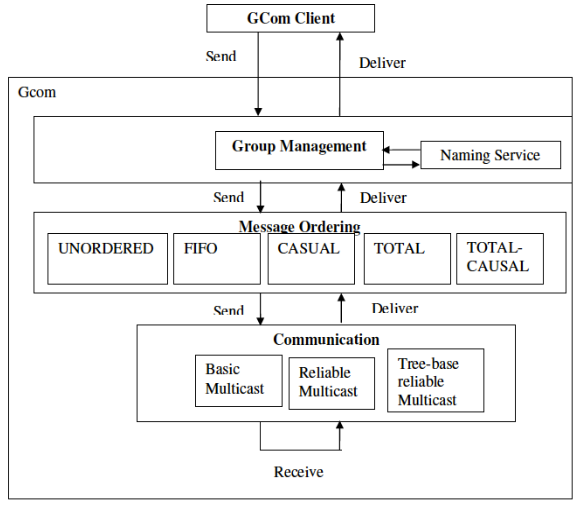
\includegraphics[width=0.7\textwidth]{figures/gcom_architecture.png}
	\end{center}
	\caption{Global architecture of GCom middleware}
	\label{fig:architecture}
\end{figure}

\paragraph{Group management}{
	The top layer is the part tasked with the group management.
 The group management elects a new leader, adds and removes
 members within the group, handles errors and notify processes
 about group changes. It is at this level a member of a group keeps
 track of other members. }

\paragraph{Message ordering}{
	The message ordering layer determines in which order
 messages are delivered to the next layer according to different
 strategies. For instance, we can order messages according to the
 "First In, First out" policy, use a causal order or a mix
 between two existing ordering like Total-Casual.
}

\paragraph{Communication}{
	The communication service is the lowest level. It deals
 with the Java RMI objects. It allows different type of
 communication like multicasting and, maybe, a tree based
 communication.  \newline
 Moreover, the debug interface will be mainly implemented here.
}

\paragraph{Debugging}{
	Additionally, the communication module offers an interface
 to set up how to simulate network latency and failures.
}

\paragraph{Naming service}{
	To get into the group, or at least ask to group to join,
 we need a service to solve how to find a group on the network.
 It is basically the entry point of the system.
 This is also the only centralized part of the system.
}

\Subsection{Comments}
	For the group management level it is important to consider
 how many members to keep track of in order to maintain
 scalability. Our first approach will be to hold all members
 but if time allows a solution where only a partial list is kept
 will be considered.

The implementation will be constructed such that every layer
as presented in above will be represented in the implementation
where no component knows of components on a layer above.
This way we keep modularity and simplicity.
Along with this, errors should propagate upwards until it can
be handled in a correct way. For example, a timeout in the 
communication layer should propagate to the group management layer
in order to e.g. inform others of a crashed member.

A final note for the structure of the product.
As Gcom is a middleware this will be built as an independent JAR
dependency so that when the chat application is constructed
Gcom acts as an external dependency imported as a JAR.
This will also make for a cleaner design and implementation
if these are properly separated.


\end{document}
